\chapter{Thuật toán BFS (Breadth-first Search)}

\minitoc

\section{Nguồn tài nguyên}

Nội dung bài chủ yếu tham khảo/copy từ [VNOI WIKI]: \url{https://wiki.vnoi.info/algo/graph-theory/breadth-first-search.md}


\section{Thuật toán duyệt đồ thị ưu tiên chiều rộng}

Thuật toán \textbf{duyệt đồ thị ưu tiên chiều rộng} (\textit{Breadth-first search} - BFS) là một trong những thuật toán tìm kiếm cơ bản và thiết yếu trên đồ thị. Trong đó, những đỉnh nào gần đỉnh xuất phát hơn sẽ \textbf{được duyệt trước}.

Ứng dụng của \textit{BFS} có thể giúp ta giải quyết tốt một số bài toán trong thời gian và không gian \textbf{tối thiểu}. Đặc biệt là bài toán tìm kiếm đường đi ngắn nhất từ một đỉnh gốc tới tất cả các đỉnh khác. Trong đồ thị không có trọng số hoặc tất cả trọng số bằng nhau, thuật toán sẽ luôn trả ra đường đi ngắn nhất có thể. Ngoài ra, thuật toán này còn được dùng để tìm các thành phần liên thông của đồ thị, hoặc kiểm tra đồ thị hai phía, \ldots

\begin{figure}[h]
    \centering
    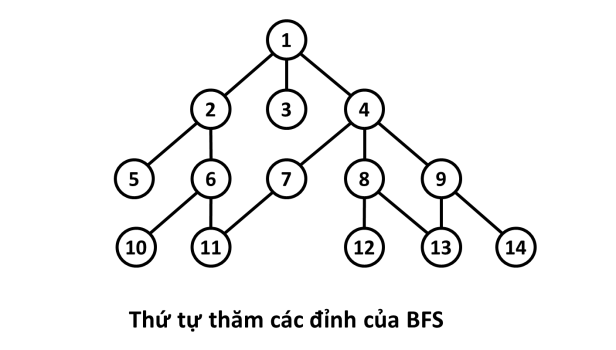
\includegraphics[width=0.4\textwidth]{resource/img/b6/breadth-first-search_img1.png}
    \caption{Thứ tự thăm các đỉnh của BFS}
\end{figure}

\subsection{Ý tưởng}

Với đồ thị không trọng số và đỉnh nguồn $s$. Đồ thị này có thể là đồ thị có hướng hoặc vô hướng, điều đó \textbf{không quan trọng} đối với thuật toán. 

Có thể hiểu thuật toán như một ngọn lửa lan rộng trên đồ thị:

\begin{itemize}
    \item Ở bước thứ $0$, chỉ có đỉnh nguồn $s$ đang cháy.
    \item Ở mỗi bước tiếp theo, ngọn lửa đang cháy ở mỗi đỉnh lại lan sang tất cả các đỉnh kề với nó.
\end{itemize}

Trong mỗi lần lặp của thuật toán, ``vòng lửa'' lại lan rộng ra theo chiều rộng. Những đỉnh nào gần $s$ hơn sẽ bùng cháy trước.

Chính xác hơn, thuật toán có thể được mô tả như sau:
\begin{itemize}
    \item Đầu tiên ta thăm đỉnh nguồn $s$.
    \item Việc thăm đỉnh $s$ sẽ phát sinh thứ tự thăm các đỉnh $(u_1, u_2, \ldots, u_p)$ kề với $s$ (những đỉnh gần $s$ nhất). Tiếp theo, ta thăm đỉnh $u_1$, khi thăm đỉnh $u_1$ sẽ lại phát sinh yêu cầu thăm những đỉnh $(v_1, v_2, \ldots, v_q)$ kề với $u_1$. Nhưng rõ ràng những đỉnh $v$ này ``xa'' $s$ hơn những đỉnh $u$ nên chúng chỉ được thăm khi tất cả những đỉnh $u$ đều đã được thăm. Tức là thứ tự thăm các đỉnh sẽ là: $s, u_1, u_2, \ldots, u_p, v_1, v_2, \ldots, v_q, \ldots$
\end{itemize}

\begin{figure}[h]
    \centering
    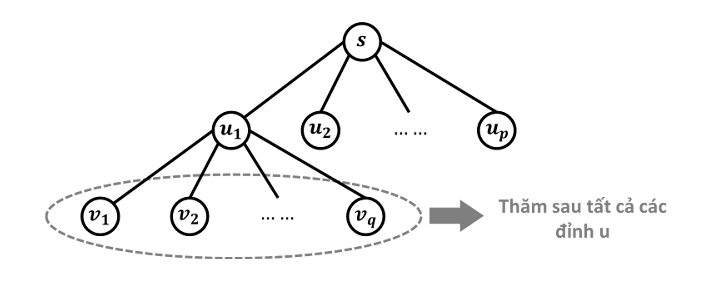
\includegraphics[width=0.5\textwidth]{resource/img/b6/breadth-first-search_img2.png}
\end{figure}

Thuật toán tìm kiếm theo chiều rộng sử dụng một danh sách để chứa những đỉnh đang ``chờ'' thăm. Tại mỗi bước, ta thăm một đỉnh đầu danh sách, loại nó ra khỏi danh sách và cho những đỉnh kề với nó chưa được thăm xếp hàng vào cuối danh sách. Thuật toán sẽ kết thúc khi danh sách rỗng.

\subsection{Thuật toán}

Thuật toán sử dụng một cấu trúc dữ liệu hàng đợi (\textit{queue}) để chứa các đỉnh sẽ được duyệt theo thứ tự ưu tiên chiều rộng.

\textbf{Bước 1: Khởi tạo}
\begin{itemize}
    \item Các đỉnh đều ở trạng thái chưa được đánh dấu. Ngoại trừ đỉnh nguồn $s$ đã được đánh dấu.
    \item Một hàng đợi ban đầu chỉ chứa 1 phần tử là $s$.
\end{itemize}

\textbf{Bước 2: Lặp lại các bước sau cho đến khi hàng đợi rỗng:}
\begin{itemize}
    \item Lấy đỉnh $u$ ra khỏi hàng đợi.
    \item Xét tất cả những đỉnh $v$ kề với $u$ mà chưa được đánh dấu, với mỗi đỉnh $v$ đó:
    \begin{itemize}
        \item Đánh dấu $v$ đã thăm.
        \item Lưu lại vết đường đi từ $u$ đến $v$.
        \item Đẩy $v$ vào trong hàng đợi (đỉnh $v$ sẽ chờ được duyệt tại những bước sau).
    \end{itemize}
\end{itemize}

\textbf{Bước 3:} Truy vết tìm đường đi.

\subsection{Mô tả}

\begin{itemize}
    \item Xét đồ thị sau đây, với đỉnh nguồn $s = 1$:
\end{itemize}

\begin{figure}[h]
    \centering
    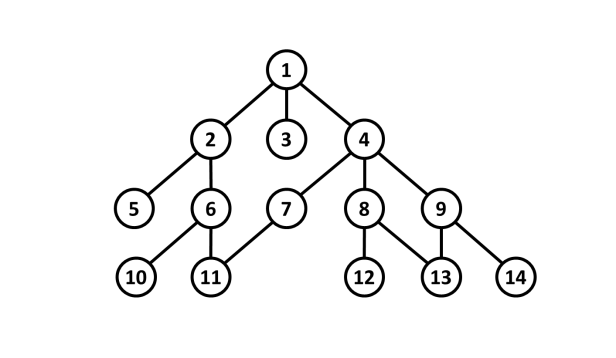
\includegraphics[width=0.5\textwidth]{resource/img/b6/breadth-first-search_img3.png}
\end{figure}
\begin{figure}[h]
    \centering
    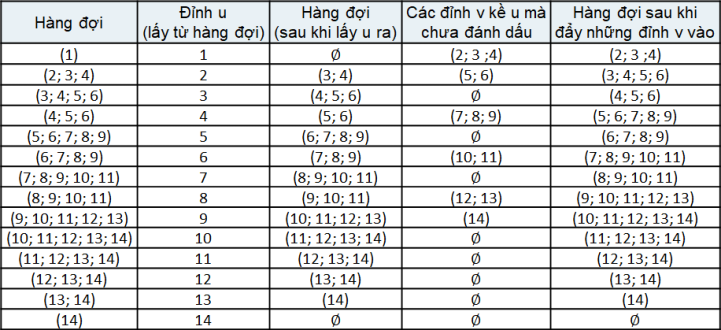
\includegraphics[width=0.5\textwidth]{resource/img/b6/breadth-first-search_img4.png}
\end{figure}

\subsection{Cài đặt}

\textbf{Cấu trúc dữ liệu:}
\begin{itemize}
    \item \texttt{n}: Số lượng đỉnh của đồ thị.
    \item \texttt{const int MAXN = 100005}: Kích thước tối đa cho các mảng.
    \item \texttt{vector<int> dist}: Mảng lưu khoảng cách (số bước) ngắn nhất từ đỉnh nguồn đến các đỉnh.
    \item \texttt{vector<int> parent}: Mảng lưu lại ``cha'' (đỉnh trước đó) trên đường đi ngắn nhất từ nguồn đến mỗi đỉnh.
    \item \texttt{vector<bool> visited}: Mảng đánh dấu các đỉnh đã được thăm.
    \item \texttt{vector<int> adj[MAXN]}: Danh sách kề (adjacency list) của mỗi đỉnh.
\end{itemize}

\begin{lstlisting}[language=C++, caption={Cài đặt}]
int n; 
const int MAXN = 100005;
vector<int> dist(MAXN, 0), parent(MAXN, -1);
vector<bool> visited(MAXN, false);
vector <int> adj[MAXN];

void bfs(int s) { 
    queue <int> q;
    q.push(s);
    visited[s] = true;
    while (q.empty() == false) {
        int u = q.front();
        q.pop();
        for (auto v : adj[u]) {
            if (visited[v] == false) {
                dist[v] = dist[u] + 1;
                parent[v] = u;
                visited[v] = true;
                q.push(v);
            }
        }
    }
}
\end{lstlisting}

\textbf{Truy vết:}
\begin{lstlisting}[language=C++, caption={Cài đặt truy vết đường đi từ đỉnh nguồn $s$ đến đỉnh $u$}]
if (visited[u] == false) {
    cout << "No path!";
} else {
    vector<int> path;
    for (int v = u; v != -1; v = parent[v])
        path.push_back(v);
    reverse(path.begin(), path.end());

    cout << "Path: ";
    for (auto v : path) cout << v << ' ';
}
\end{lstlisting}

\subsection{Các đặc tính của thuật toán}

Nếu sử dụng một ngăn xếp (\textit{stack}) thay vì hàng đợi (\textit{queue}) thì ta sẽ thu được \textbf{thứ tự duyệt đỉnh} của thuật toán \textbf{tìm kiếm theo chiều sâu} (\textit{Depth First Search} -- DFS). Đây chính là \textbf{phương pháp khử đệ quy} của DFS để cài đặt thuật toán trên các ngôn ngữ không cho phép đệ quy.

\textbf{Định lý:} Thuật toán \textit{BFS} cho ta độ dài đường đi ngắn nhất từ đỉnh nguồn tới mọi đỉnh (với khoảng cách tới đỉnh $u$ bằng $d[u]$).  
Trong thuật toán \textit{BFS}, nếu đỉnh $u$ xa đỉnh nguồn hơn đỉnh $v$, thì $u$ sẽ được thăm sau $v$.

\begin{itemize}
    \item \textbf{Chứng minh:} Trong \textit{BFS}, từ một đỉnh hiện tại, ta luôn đi thăm tất cả các đỉnh kề với nó trước, sau đó thăm tất cả các đỉnh cách nó một đỉnh, rồi các đỉnh cách nó hai đỉnh, v.v... Như vậy, nếu từ một đỉnh $u$ khi ta chạy \textit{BFS}, quãng đường đến đỉnh $v$ luôn là quãng đường đi qua ít cạnh nhất.
\end{itemize}

\subsection{Định lý Bắt tay (Handshaking lemma)}

\textbf{Định lý:} Trong một đồ thị bất kỳ, tổng số bậc của tất cả các đỉnh bằng \textbf{gấp đôi} số cạnh của đồ thị.

\textbf{Mô tả:} Cho đồ thị $G = (V, E)$ gồm $|V|$ đỉnh và $|E|$ cạnh. Khi đó, tổng tất cả các bậc của đỉnh trong $G$ bằng $2 \times |E|$.  
Với $\deg(v)$ là số bậc của đỉnh $v$, có:
\[
\sum_{v \in V} \deg(v) = 2 \times |E|
\]

\textbf{Ví dụ:} Cho đồ thị sau với $|V| = 8$ và $|E| = 7$:

\begin{figure}[h]   
    \centering
    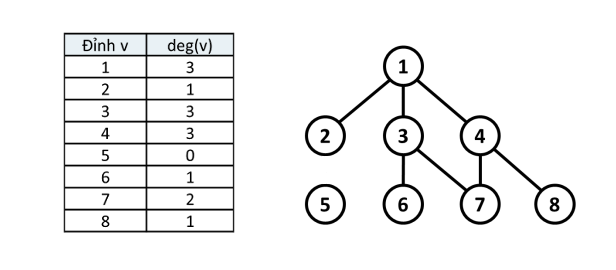
\includegraphics[width=0.5\textwidth]{resource/img/b6/breadth-first-search_img5.png}
\end{figure}

\[
\sum_{v \in V} \deg(v) = 2 \times |E| = 2 \times 7 = 14
\]

\textbf{Chứng minh:}  
Vì mỗi một cạnh nối với đúng hai đỉnh của đồ thị, nên một cạnh sẽ đóng góp $2$ đơn vị vào tổng số bậc của tất cả các đỉnh.

\textbf{Hệ quả:} Trong đồ thị, số lượng \textbf{đỉnh bậc lẻ} luôn là một số chẵn.

\textbf{Chứng minh:} Gọi $L$ và $C$ lần lượt là tập các đỉnh bậc lẻ và bậc chẵn của đồ thị $G=(V,E)$. Ta có:
\[
2 \times |E| = \sum_{v \in V} \deg(v) = \sum_{v \in C} \deg(v) + \sum_{v \in L} \deg(v)
\]
$2 \times |E|$ là số chẵn $\implies \sum_{v \in C} \deg(v)$ chẵn, $\sum_{v \in L} \deg(v)$ chẵn $\implies$ số phần tử của $L$ là chẵn.

\textbf{Nhận xét:}
\begin{itemize}
    \item Trong quá trình duyệt đồ thị được biểu diễn bằng \textbf{danh sách kề}, mỗi cạnh sẽ được duyệt chính xác hai lần đối với \textbf{đồ thị vô hướng} (vì mỗi cạnh sẽ được lưu trong 2 danh sách kề của 2 đỉnh). Còn đối với \textbf{đồ thị có hướng}, mọi cạnh của đồ thị chỉ được duyệt chính xác một lần.
\end{itemize}

\textbf{Tham khảo:} \href{https://en.wikipedia.org/wiki/Handshaking_lemma}{Handshaking\_lemma}

\subsection{Độ phức tạp thuật toán}

\paragraph{Độ phức tạp thời gian}

Gọi $|V|$ là số lượng đỉnh và $|E|$ là số lượng cạnh của đồ thị.

Trong quá trình \textit{BFS}, cách biểu diễn đồ thị có ảnh hưởng lớn tới chi phí về thời gian thực hiện giải thuật:

\begin{itemize}
    \item \textbf{Nếu đồ thị biểu diễn bằng danh sách kề} (\texttt{vector g[]}):

    \begin{itemize}
        \item Ta có thể thực hiện thuật toán này một cách tối ưu nhất về mặt thời gian nhờ khả năng duyệt qua các đỉnh kề của mỗi đỉnh một cách hiệu quả.
        \item Vì ta sử dụng mảng \texttt{visited[]} để ngăn việc đẩy một đỉnh vào hàng đợi nhiều lần nên mỗi đỉnh sẽ được thăm \textbf{chính xác một lần} duy nhất. Do đó, ta mất độ phức tạp thời gian $O(|V|)$ cho việc thăm các đỉnh.
        \item Bất cứ khi nào một đỉnh được thăm, mọi cạnh kề với nó đều được duyệt, với thời gian dành cho mỗi cạnh là $O(1)$. Từ nhận nhận xét của định lý Bắt tay (\textit{Handshaking lemma}), ta sẽ mất độ phức tạp thời gian $O(|E|)$ dành cho việc duyệt các cạnh.
        \item Nhìn chung, độ phức tạp thời gian của thuật toán là $O(|V| + |E|)$. Đây là cách cài đặt tối ưu nhất.
    \end{itemize}

    \item \textbf{Nếu như đồ thị được biểu diễn bằng ma trận kề:}
    \begin{itemize}
        \item Ta cũng sẽ mất độ phức tạp thời gian $O(|V|^2)$ cho việc thăm các đỉnh (giải thích tương tự như trên).
        \item Với mỗi đỉnh được thăm, ta phải duyệt qua toàn bộ các đỉnh của đồ thị để kiểm tra đỉnh kề với nó. Do đó, thuật toán sẽ mất độ phức tạp $O(|V|^2)$.
    \end{itemize}
\end{itemize}

\paragraph{Độ phức tạp không gian}
Tại mọi thời điểm, trong hàng đợi (\texttt{queue q}) có không quá $|V|$ phần tử. Do đó, độ phức tạp bộ nhớ là $O(|V|)$.

\section{Ứng dụng BFS để xác định thành phần liên thông}

\begin{baitap}{BDFS - Đếm số thành phần liên thông}{https://lequydon.ntucoder.net/Problem/Details/4601}
Cho đơn đồ thị vô hướng gồm $n$ đỉnh và $m$ cạnh ($1 \leq n, m \leq 10^5$), các đỉnh được đánh số từ $1$ tới $n$. Tìm số \textbf{thành phần liên thông} của đồ thị.

\subsection{Ý tưởng}

Một đồ thị có thể liên thông hoặc không liên thông. Nếu đồ thị liên thông thì số thành phần liên thông của nó là $1$. Điều này tương đương với phép duyệt theo thủ tục \textit{BFS} được gọi đến đúng một lần. Nếu đồ thị không liên thông (số thành phần liên thông lớn hơn $1$), ta có thể tách chúng thành những \textbf{đồ thị con liên thông}. Điều này cũng có nghĩa là trong phép duyệt đồ thị, số thành phần liên thông của nó bằng số lần gọi tới thủ tục \textit{BFS}.

\subsection{Thuật toán}

Thuật toán ứng dụng \textit{BFS} để xác định thành phần liên thông:

\begin{itemize}
    \item \textbf{Bước 0:} Khởi tạo số lượng thành phần liên thông bằng $0$.
    \item \textbf{Bước 1:} Xuất phát từ một đỉnh chưa được đánh dấu của đồ thị. Ta đánh dấu đỉnh xuất phát, tăng số thành phần liên thông thêm $1$.
    \item \textbf{Bước 2:} Từ một đỉnh đã đánh dấu, đánh dấu tất cả các đỉnh $j$ kề với $i$ mà $j$ chưa được đánh dấu.
    \item \textbf{Bước 3:} Thực hiện bước 2 cho đến khi không còn đỉnh nào được nữa.
    \item \textbf{Bước 4:} Nếu số đỉnh chưa đánh dấu (mảng \texttt{visited} chưa đánh dấu) kết thúc thuật toán và trả về số thành phần liên thông, ngược lại quay về bước 1.
\end{itemize}
\end{baitap}

\paragraph{Cài đặt, độ phức tạp O(N + M)}
\begin{lstlisting}[language=C++]
#include <bits/stdc++.h>
#define int long long
#define endl "\n"
using namespace std;

int n, m, componentNumber = 0; 
const int MAXN = 100005;
vector<bool> visited(MAXN, false);
vector <int> adj[MAXN];

void bfs(int s) { 
    queue <int> q;
    q.push(s);
    visited[s] = true;
    while (q.empty() == false) {
        int u = q.front();
        q.pop();
        for (auto v : adj[u]) {
            if (visited[v] == false) {
                dist[v] = dist[u] + 1;
                parent[v] = u;
                visited[v] = true;
                q.push(v);
            }
        }
    }
    componentNumber++;
}

signed main() {
    cin >> n >> m;
    for (int i = 1; i <= m; i++) {
        int u, v; cin >> u >> v;
        adj[u].push_back(v);
        adj[v].push_back(u);
    }
    for (int u = 1; u <= n; u++) {
        if (visited[u] == false) {
            bfs(u);
        }
    }
    cout << componentNumber;
}
\end{lstlisting}

\section{Ứng dụng BFS để tìm đường đi ngắn nhất trong đồ thị có trọng số 0 hoặc 1}

\begin{baitap}{REVERSE - Chef and Reversing}{https://site.ada.edu.az/~medv/acm/Docs\%20Codechef/2014/August\%20Challenge\%202014/reverse.htm}

Cho một đồ thị có hướng $N$ đỉnh và $M$ cạnh ($1 \leq N, M \leq 10^5$). Tìm số cạnh ít nhất cần phải đảo chiều để tồn tại đường đi từ đỉnh 1 cho đến đỉnh $N$.

Các đỉnh được đánh số từ $1$ đến $N$. Đồ thị có thể có nhiều cạnh nối giữa một cặp đỉnh. Và có thể tồn tại cạnh nối từ một đỉnh đến chính nó (\textit{đồ thị có thể có khuyên}).

\subsection{Phân tích}

Gọi đồ thị ban đầu là $G$.

Ta sẽ thêm các \textbf{cạnh ngược} của mỗi cạnh ban đầu trong đồ thị $G'$ (nghĩa là, với mỗi cạnh $u \to v$ của đồ thị, ta sẽ thêm cạnh $v \to u$ vào).  
Cho các cạnh ngược có trọng số bằng $1$ và tất cả các cạnh ban đầu có trọng số bằng $0$. Khi đó, ta sẽ có được đồ thị mới là đồ thị $G'$.

Độ dài của đường đi ngắn nhất từ đỉnh $1$ cho đến đỉnh $N$ trong đồ thị $G'$ chính là đáp án của bài toán.

\begin{itemize}
    \item \textbf{Chứng minh:} Trong đồ thị $G'$, xét từng cạnh trên một đường đi từ $1$ đến $N$. Nếu cạnh đó có trọng số là $0$ thì đã tồn tại cạnh đó trên đồ thị $G$ ban đầu, nếu trọng số là $1$ thì cạnh ngược này cần tạo trong đồ thị $G$, khi đó phải đảo chiều cạnh đó. Nhận thấy sau khi xét toàn bộ các cạnh, ta sẽ thu được một đường đi từ $1$ đến $N$, và số cạnh bị phải đảo chiều chính là số cạnh $1$ trong đường đi đó.
\end{itemize}

Ta sử dụng \textbf{kỹ thuật 0-1 BFS}:

\begin{itemize}
    \item Nó có tên gọi như vậy vì kỹ thuật \textbf{0-1 BFS} thường được sử dụng để tìm đường đi ngắn nhất trong đồ thị có trọng số $0$ hoặc $1$.
    \item Khi trọng số của các cạnh bằng $0$ hoặc $1$, thuật toán \textit{BFS} thông thường sẽ trả ra kết quả sai, vì thuật toán \textit{BFS} thông thường chỉ đúng trong đồ thị có trọng số của các cạnh bằng nhau.
\end{itemize}
Ta có thể chỉnh sửa một chút từ thuật toán \textit{BFS} để có được \textbf{kĩ thuật 0-1 BFS}:

\begin{itemize}
    \item Trong kĩ thuật này, thay vì sử dụng mảng \texttt{bool} để đánh dấu lại các đỉnh đã duyệt, ta sẽ kiểm tra điều kiện \textbf{khoảng cách ngắn nhất}. Nghĩa là, trong quá trình \textit{BFS}, với mỗi đỉnh $v$ kề với $u$, đỉnh $v$ chỉ được đẩy vào hàng đợi khi và chỉ khi đường đi đi ngắn nhất từ đỉnh nguồn đến $v$ lớn hơn đường đi ngắn nhất từ đỉnh nguồn đến $u$ cộng với trọng số cạnh $u \rightarrow v$ (khoảng cách được giảm bớt khi sử dụng cạnh này).
    \item Ta sẽ sử dụng một \textbf{hàng đợi hai đầu} \href{https://wiki.vnoi.info/algo/data-structures/Deque}{(\textit{deque})} thay cho hàng đợi (\textit{queue}) để lưu trữ các đỉnh. Trong quá trình \textit{BFS}, nếu ta gặp một cạnh có trọng số bằng $0$ thì đỉnh sẽ được đẩy vào \textbf{phía trước} của hàng đợi hai đầu. Ngược lại, nếu ta gặp một cạnh có trọng số bằng $1$ thì đỉnh sẽ được đẩy vào \textbf{phía sau} của hàng đợi hai đầu.
    \begin{itemize}
        \item \textbf{Giải thích:} Ta push đỉnh kề nổi bởi cạnh có trọng số $0$ vào \texttt{deque} để giữ cho hàng đợi luôn được sắp xếp theo khoảng cách từ đỉnh nguồn tại mọi thời điểm. Bởi vì, các đỉnh có quãng đường đi gần queue/deque hơn thì nó phải có khoảng cách từ gốc gần hơn, nên ta thêm ta \texttt{push} vào đầu tức khoảng cách chính khoảng cách đỉnh vừa \texttt{pop} ra, nên \texttt{deque} lúc này thỏa mãn tính chất của \texttt{queue} trong \textit{BFS}.
    \end{itemize}
    \item Từ tính chất trên, ta có nhận xét sau: \textbf{Kĩ thuật 0-1 BFS} vẫn đúng cho trường hợp đồ thị có trọng số cạnh là $0$ hoặc $x$ ($x \geq 0$).
\end{itemize}

Cách tiếp cận của \textbf{kĩ thuật 0-1 BFS} khá giống với thuật toán \textit{BFS} + \href{https://en.wikipedia.org/wiki/Dijkstra%27s_algorithm}{Dijkstra}.

\end{baitap}

\paragraph{Cài đặt, độ phức tạp $O(M + N)$}
\begin{lstlisting}[language=C++]
#include <bits/stdc++.h>
#define int long long
#define endl "\n"
using namespace std;

const int oo = 1e18;
const int MAXN = 100005;

int n, m;
int dist[MAXN];
vector <pair<int, int>> adj[MAXN];

void bfs(int s) {
    for (int i = 1; i <= n; i++) dist[i] = oo;
    deque <int> q;
    q.push_back(s);
    dist[s] = 0;
    while (q.empty() == false) {
        int u = q.front();
        q.pop_front();
        if (u == n) break;
        for (auto edge : adj[u]) {
            int w = edge.first;
            int v = edge.second;
            if (dist[v] > dist[u] + w) {
                dist[v] = dist[u] + w;
                if (w == 0) q.push_front(v);
                else q.push_back(v);
            }
        }
    }
    if (dist[n] == oo) dist[n] = -1;
}

signed main() {
    cin >> n >> m;
    for (int i = 1; i <= m; i++) {
        int u, v; cin >> u >> v;
        adj[u].push_back({0, v});
        adj[v].push_back({1, u});
    }
    bfs(1);
    cout << dist[n];
}
\end{lstlisting}